\section{Introduction}
\label{sec:intro}

Agent applications solve tasks through sequences of dependent LLM calls that repeatedly consume common context, including instructions, input documents, and intermediate results. Yet repeated content does not automatically translate into reusable computation. Processing a prompt, known as \emph{prefill}, produces attention states stored in a key-value (KV) cache. A serving system can reuse these states when a later prompt begins with the same sequence of tokens, called a \emph{shared prefix}. The remaining portion of the prompt is its \emph{suffix}.

Whether reuse improves performance also depends on cache management. GPU memory is limited, and retaining cached states for one call can displace states needed by another. Evicting a prefix before its next use forces recomputation, while retaining context that will not be reused wastes scarce memory. Under KV-cache thrashing, per-request prefill time can grow by $6.8\times$ and generation throughput can drop by up to 66\%~\cite{yuan2026agentic}. Efficient serving therefore requires both exposing reusable prefixes and deciding which cached states deserve memory between calls.

Existing systems exploit prefix sharing and workflow predictability. SGLang's RadixAttention reuses the longest cached prefix matching each incoming prompt and prioritizes requests with longer matches~\cite{zheng2024sglang}. Workflow-aware systems such as KVFlow, Helium, PBKV, and CacheScout~\cite{pan2025kvflow,wadlom2026helium,zheng2026pbkv,zhang2026cachescout} use workflow structure or observed execution patterns to anticipate upcoming calls and guide cache management. KVFlow, for example, uses predicted agent execution order to prioritize retention of fixed prompt prefixes, while assigning varying suffixes the highest eviction priority. This policy treats the suffix as opaque with respect to its components' reuse potential: it does not distinguish persistent shared values from temporary content within that suffix.

\textbf{However, we observe that the dynamic suffix has internal structure: it comprises distinct components with different sharing patterns and lifetimes, a property we term intra-prompt heterogeneity.} A session-wide input, an accumulating history, and a temporary result may appear together in one prompt, yet have very different reuse potential. Some values recur across several calls, some preserve earlier content as they grow, and others cease to be needed after a single iteration. Recognizing this structure creates opportunities to expose sharing hidden by the current prompt order and to distinguish useful cached states from those that can be released.

\begin{figure}[h]
    \centering
    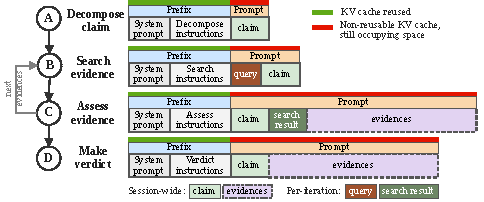
\includegraphics[width=1.0\linewidth]{figures/before.pdf}
    \caption{Original prompt layouts for a fact-checking agent. Call-specific instructions precede shared context, limiting prefix reuse across call sites. The claim remains unchanged, evidence accumulates, and queries and individual search results are replaced between iterations.}
    \label{fig:original-view}
    \vspace{-10pt}
\end{figure}

Consider the fact-checking agent in Figure~\ref{fig:original-view}. Given a claim, the agent generates a query (A), searches for evidence (B), and assesses the result against previously collected evidence (C). It repeats the search and assessment until it can produce a verdict (D). In this example, prior systems reuse fixed instruction prefixes consisting of the common system prompt followed by the instructions for decomposition (A), search (B), assessment (C), or verdict generation (D). Their cache retention and eviction policies manage these identified prefixes without distinguishing the sharing patterns and lifetimes of individual components in the dynamic suffix. The claim flows unchanged to all four call sites and remains useful throughout the session. The evidence collection is shared by assessment and verdict calls and preserves accumulated content as it grows. Queries and individual search results are replaced between iterations. These differences remain hidden when the dynamic suffix is treated as opaque.

\textbf{First, this structure enables prompt layouts that expose more prefix reuse.} In Figure~\ref{fig:original-view}, each call site's fixed instructions can be reused across its invocations, but the instructions differ across sites and precede the shared claim. Consequently, ordinary prefix matching cannot reach the claim across those calls. Moving the claim immediately after the common system prompt exposes a shared prefix across all four sites. Placing accumulated evidence before temporary inputs similarly exposes its unchanged token prefix for reuse in later calls. Once these prefixes are exposed, the serving engine's existing matching mechanism can reuse them.
\textbf{Second, this structure enables retention decisions based on future uses.} The claim will be consumed by later calls, whereas cached states for an iteration's temporary tails may never be reused. Figure~\ref{fig:intra-prompt} illustrates retaining shared prefixes while releasing disposable tails. Although a search result's content is appended to the evidence collection, its cached states in the original prompt position need not remain reusable. Component relationships must therefore be interpreted together with prompt order: layout determines which values form reusable prefixes, and lifecycle information helps determine how long those prefixes are worth retaining.

\begin{figure}[t]
    % \vspace{-8pt}
    \centering
    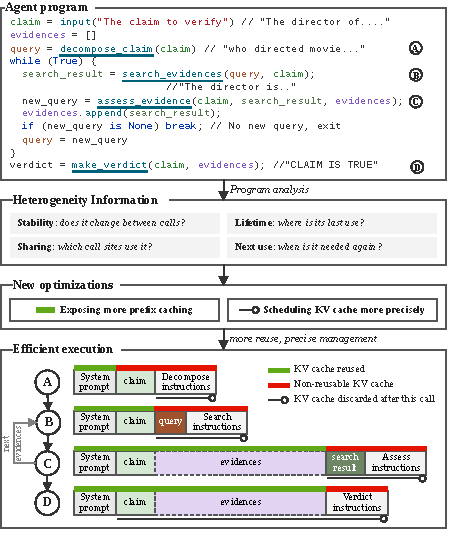
\includegraphics[width=0.85\linewidth]{figures/after.pdf}
    \caption{Program analysis recovers sharing, updates, and lifetime information for prompt components. Combined with runtime observations, this information guides coordinated prompt layouts and cache retention. Shared context moves forward, while discard markers identify cached tails that can be released after a call.}
    \label{fig:intra-prompt}
    \vspace{-8pt}
\end{figure}

\textbf{Our key insight is that the sharing patterns and lifetimes of program values provide actionable information for exposing additional prefix reuse and retaining cached states according to their future uses. More importantly, we observe that this sharing and lifetime information is already encoded in the agent program itself, making it recoverable through compiler analysis.} Frameworks such as byLLM, NOOA, and DSPy~\cite{furgale2026nooa,khattab2024dspy,dantanarayana2025mtp} generate prompts from typed LLM function declarations and argument values, establishing a correspondence between prompt components and program variables. In Figure~\ref{fig:intra-prompt}, dataflow connects the claim to all four call sites, the append operation exposes growing evidence, and assignments inside the loop identify replaced queries. Control flow identifies possible future consumers. Recovering these relationships makes it possible to coordinate layouts across calls and reason about the future usefulness of their cached states, even before those future prompts arrive.

Turning this insight into efficient serving requires addressing three challenges. \textbf{First, program structure alone does not determine actual reuse.} Static analysis reveals possible sharing, updates, and future consumers, but execution paths, component sizes, and inter-call delays vary at runtime. \textbf{Second, exposing prefix reuse requires coordination across call sites.} Independently ordering each call's components can place the same value behind different preceding contexts, preventing its cached states from being shared. \textbf{Third, potential reuse must be weighed against current memory demand.} Retaining or prefetching a prefix for a future call consumes memory that other requests could use, while premature eviction forces recomputation.

We present \sysname, a co-design of the compiler and serving runtime that addresses these challenges through a common description of prompt components and their uses. To connect program structure with actual execution, the compiler produces component metadata and a workflow graph, which the runtime supplements with observations to estimate future reuse and its timing. Using this information, \emph{adaptive prompt re-layout} coordinates component ordering across related calls to expose longer shared prefixes. \emph{Proactive KV-cache scheduling} then uses component lifetimes and predicted reuse to prioritize retention and eviction. It bounds retention with a fixed memory budget and prefetches only into available space, reclaiming disposable cached tails when needed. Together, these mechanisms connect the analysis of program values to both the construction of reusable prefixes and the allocation of memory to preserve them.

We make the following contributions:
\begin{enumerate*}[label=\textbf{(\roman*)}]
    \item We identify intra-prompt heterogeneity and the opportunities it creates to expose additional prefix reuse and distinguish the retention needs of prompt components.
    \item We develop a compiler analysis methodology that recovers component sharing and lifetimes from agent programs and combines this information with runtime observations to coordinate prompt layout and cache management.
    \item We implement \sysname and evaluate it on four agent workloads. It achieves geometric-mean speedups of 1.45$\times$ in average job completion time (JCT) and 1.49$\times$ in throughput over SGLang, with maxima of 1.99$\times$ and 1.97$\times$, respectively.
\end{enumerate*}
